\documentclass[a4paper]{article}
\usepackage[pdftex]{graphicx}
\usepackage[utf8]{inputenc}
\usepackage{enumerate}
\usepackage{amssymb}
\usepackage{eurosym}
\usepackage{icomma}
\usepackage{siunitx}
\sisetup{locale=DE} 
\usepackage{tikz}
\usepackage{href-ul}
\hypersetup{
	colorlinks=true,
	linkcolor=blue,
	urlcolor=blue}
\usepackage{geometry}
\geometry{a4paper, top=15mm, left=15mm, right=15mm, bottom=15mm,
	headsep=10mm, footskip=12mm}

\begin{document}
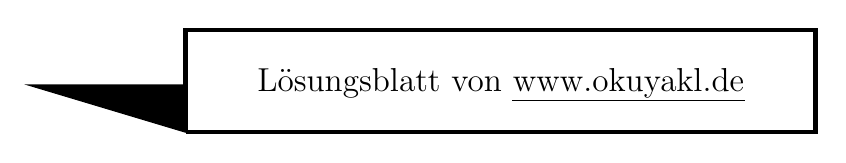
\begin{tikzpicture}(10,3)
	\draw[ultra thick](2,0) --(10,0) -- (10,1.3) --(2,1.3) -- (2,0);
	\draw[fill=black](2,0)-- (0,.6) -- (2,.6) -- (2,0);
	\node at (6,.6) {\large Lösungsblatt von \href{https://www.okuyakl.de}{www.okuyakl.de}};
\end{tikzpicture}
\vspace{0.5 cm}

\renewcommand{\arraystretch}{2.5}
\begin{tabular}{|c|p{13 cm}|}
\hline
$< \SI{1000}{\meter^3}$ & Mehrfamilienhaus\\
\hline
$\SI{100}{\meter^3}$ bis $\SI{1000}{\meter^3}$ & 50-m-Schwimmbecken\\
\hline
$\SI{10}{\meter^3}$ bis $\SI{100}{\meter^3}$ & Klassenzimmer\\
\hline
$\SI{1}{\meter^3}$ bis $\SI{10}{\meter^3}$ & Tanklastwagen, Glascontainer\\
\hline
$\SI{100}{\deci\meter^3}$ bis $\SI{1}{\meter^3}$ & Badewanne, Kajak \\
\hline
$\SI{10}{\deci\meter^3}$ bis $\SI{100}{\deci\meter^3}$ & Auto-Tank\\
\hline
$\SI{1}{\deci\meter^3}$ bis $\SI{10}{\deci\meter^3}$ & Benzinkanister, Fußball\\
\hline
$\SI{100}{\centi\meter^3}$ bis $\SI{1}{\deci\meter^3}$ & Trinkglas, Flasche\\
\hline
$\SI{10}{\centi\meter^3}$ bis $\SI{100}{\centi\meter^3}$ & Tischtennisball, Osterei\\
\hline
$\SI{1}{\centi\meter^3}$ bis $\SI{10}{\centi\meter^3}$ & Spielwürfel, Daumen\\
\hline
$\SI{100}{\milli\meter^3}$ bis $\SI{1}{\centi\meter^3}$ & Fingerhut, Tintenpatrone\\
\hline
$\SI{10}{\milli\meter^3}$ bis $\SI{100}{\milli\meter^3}$ & Weizenkorn, Streichholzkopf\\
\hline
$\SI{1}{\milli\meter^3}$ bis $\SI{10}{\milli\meter^3}$ & Regentropfen, Schrotkorn\\
\hline
$< \SI{1}{\milli\meter^3}$ & Mohnsamen, Sandkorn\\
\hline
\end{tabular}

\begin{center}
	\includegraphics[width=7 cm]{../../viecher/endcomic.pdf}
	
	Hier geht es zurück zum \href{https://www.okuyakl.de/phys/p7vgrL066/aa066.pdf}{Aufgabenblatt}
\end{center}

\end{document}

